\documentclass{article} 

\usepackage{amsmath,amsthm}  

\usepackage{mathtools} 
\usepackage{graphicx}     
%\usepackage{hyperref} 
%\usepackage{url}
\usepackage{amsfonts} 
\usepackage{multicol}

\newtheorem{theorem}{Theorem}[section]
\newtheorem{corollary}{Corollary}[theorem]
\newtheorem{lemma}[theorem]{Lemma}

\theoremstyle{definition}
\newtheorem*{definition}{Definition}
\newtheorem*{remark}{Remark}

\allowdisplaybreaks

\makeatletter
\@addtoreset{footnote}{page}
\makeatother

%%%%%%%%%%%%%%%%%%%%%%%%%%%%%%%%%%%%%%%%%%%%%%%%%%
\begin{document}


\title{Extending the Hyperoperators}

\author{Daniel Geisler\\               %%
daniellgeisler@gmail.com}                    

\maketitle

\begin{abstract}
  The first three arithmetic operators - addition, multiplication, and exponentiation can be extended from the natural numbers, to the complex numbers and even the matrices of general linear groups. But extending tetration, pentation, and the higher hyperoperators requires dealing with their chaotic nature. Fa\'a Di Bruno's formula provides a combinatorial generation of the composition of functions that also applies to iterated functions and produces difference equations, whose solution are iterated functions. This is then applied to the hyperoperators whose convergence in the complex plane results from only using composition with entire functions which are convergent and closed under composition. The connection between mathematical dynamical systems and the physics they encompass is noted. [MSC 37Cxx, 11xxx, 05A17]
\end{abstract}

\section{Introduction}
A question that goes back to Poincar\'e's time is, "do maps have flows?" For a smooth function $f(x)$ and it's iterate, $f^t(x)$, what degree does $t \in \mathbb{N^+}$ imply $t \in  \mathbb{R}, \mathbb{C}$, and $\mathbb{GL}(n)$? Physics appears to do fine reconciling iterated functions and continuous time. Arnold \cite{Jackson} defines physical dynamical systems as measure preserving iterated functions acting on an initial state. The system under review is more general than any physical system as it has no constraint to be measure preserving. 

Returning to the realm of mathematics and arithmetic, let $f(x)$ and $g(x)$ be functions in Banach space, then the composite $f(g(x))$ can be constructed using Fa\'a Di Bruno's formula.

\begin{figure}
    \centering
    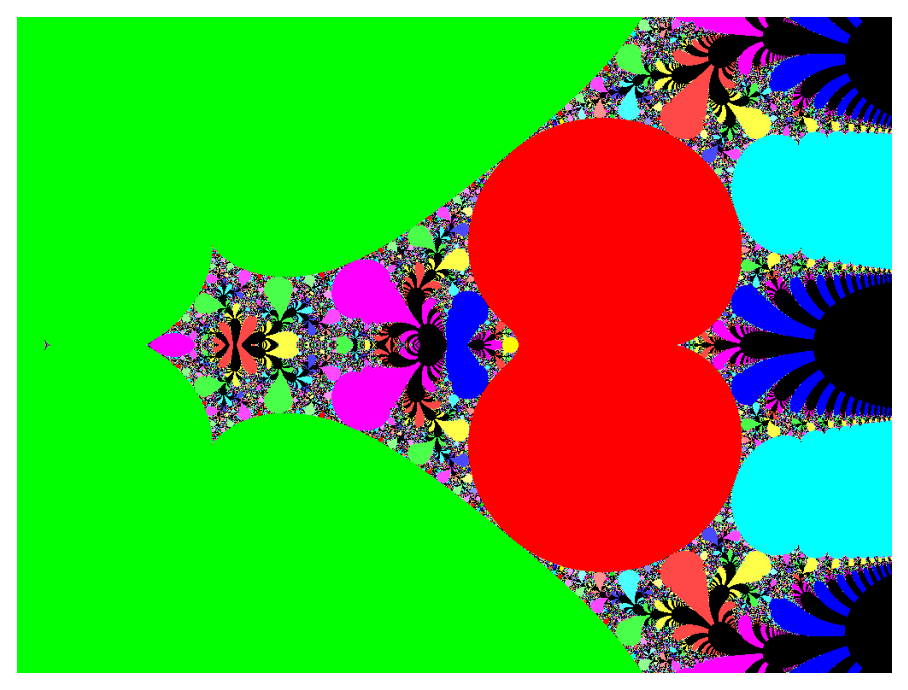
\includegraphics[width=2.5in]{Period.eps}
    \caption{Period}
    \label{fig:Period}
\end{figure}

\begin{figure}
    \centering
    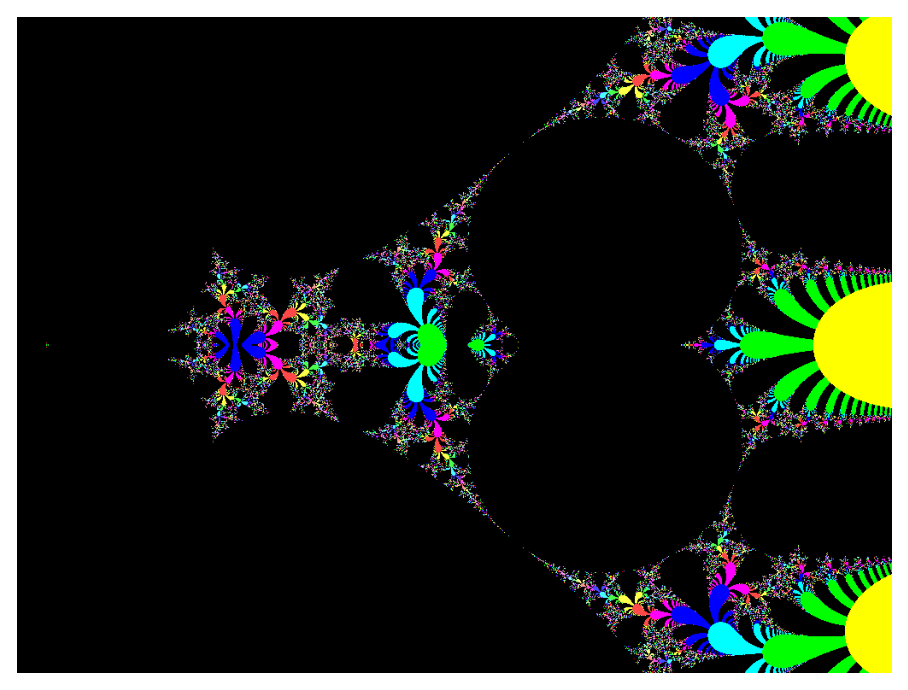
\includegraphics[width=2.5in]{Escape.eps}
    \caption{Escape}
    \label{fig:Escape}
\end{figure}

\begin{eqnarray}
D^nf(g(x)) = \sum_{\pi(n)} \frac{n!}{k_1! \cdots k_n!} 
(D^kf)(g(x))
\left(\frac{Dg(x)}{1!}\right)^{k_1} \cdots
\left(\frac{D^ng(x)}{n!}\right)^{k_n}
\label{eq:FaaDiBruno}
\end{eqnarray}
where $\pi(n)$ denotes a partition of $n$, usually denoted by $1^{k_1}2^{k_2}\cdots n^{k_n}$, with $k_1+2k_2+ \cdots nk_n=k$; where $k_i$ is the number of parts of size $i$. The partition function $p(n)$ is a decategorized version of $\pi(n)$, the function $\pi(n)$ enumerates the integer partitions of $n$, while $p(n)$ is the cardinality of the enumeration of $\pi(n)$. \cite{Comtet} \cite{Riordan}

\section{Complex Dynamics}

Now we focus on the complex plane and it's dynamics. The composition $f(g(z))$ can construct any iterated function at a fixed point, not at infinity, by setting $f(0)=0$ and $g(z)=f^{t-1}(z)$ with $t \in \mathbb{N^+}$. The final proof of this section extends $t \in \mathbb{C}$. The first derivative of $f(z)$ at its fixed point $Df(0)$ is often represented by $\lambda$ and referred to as the multiplier or the Lyapunov characteristic number; its logarithm is known as the Lyapunov exponent. 

\subsection{The First Derivative}

The first derivative results in the well known Linearization Theorem.

  \begin{eqnarray*}
  Df(g(z))&=&f'(g(z))g'(z)\\
  &=&f'(f^{t-1}(z))Df^{t-1}(z)\\
  &=&\prod^{t-1}_{k_1=0}f'(f^{t-k_1-1}(z))\\
  \end{eqnarray*} 
  \begin{eqnarray}           
  Df^t(0)&=&\lambda^t
  \label{eq:TheFirstDerivative}
  \end{eqnarray}

\subsection{The Second Derivative}  

The higher derivatives can be evaluated in an analogous fashion from the second derivative.
\begin{eqnarray}
  D^2f(g(z))&=&f''(g(z))g'(z)^2+f'(g(z))g''(z) \nonumber\\
          &=&f''(f^{t-1}(z))(Df^{t-1}(z))^2+f'(f^{t-1}(z))D^2f^{t-1}(z)
\end{eqnarray}

Setting $g(z) = f^{t-1}(z)$ results in
\begin{eqnarray}        
 D^2f^t(0)&=& f''(0) \lambda^{2t-2}+\lambda D^2f^{t-1}(0)\nonumber
\end{eqnarray}
When $\lambda \neq 0$, a recurrence equation is formed that is solved as a summation. 

\begin{eqnarray}             
 D^2f^t(0)&=&f''(0)\lambda^{2t-2}+\lambda D^2f^{t-1}(0)\nonumber\\
            &=&\lambda^0f''(0) \lambda^{2t-2}\nonumber\\
            &&+\lambda^1f''(0) \lambda^{2t-4}\nonumber\\
            &&+\cdots\nonumber\\
            &&+\lambda^{t-2}f''(0) \lambda^2\nonumber\\
            &&+\lambda^{t-1}f''(0) \lambda^0\nonumber\\
            &=&f''(0)\sum_{k_1=0}^{t-1}\lambda^{2t-k_1-2}
 \label{eq:TheSecondDerivative}            
\end{eqnarray}



\subsection{The Third Derivative}
\label{sec:TheThirdDerivative}
Continuing on with the third derivative,

\begin{eqnarray}
	D^3f(g(z))&=&f'''(g(z))g'(z)^3+3f''(g(z))g'(z)g''(z)+f'(g(z))g'''(z)\nonumber\\
	          &=&f'''(f^{t-1}(z))(Df^{t-1}(z))^3\nonumber\\
	           &&+3f''(f^{t-1}(z))Df^{t-1}(z)D^2f^{t-1}(z)\nonumber\\
	           &&+f'(f^{t-1}(z))D^3f^{t-1}(z)\nonumber
\end{eqnarray}

\begin{eqnarray}
 D^3f^t(0)&=&f_3\lambda^{3t-3}+3 f_2^2\sum_{k_1=0}^{t-1}\lambda^{3t-k_1-5}
               +\lambda D^3f^{t-1}(0) \nonumber\\
            &=&f_3\sum_{k_1=0}^{t-1}\lambda^{3t-2k_1-3}
               +3f_2^2 \sum_{k_1=0}^{t-1}
                       \sum_{k_2=0}^{t-k_1-2}
                          \lambda^{3t-2k_1-k_2-5}  
 \label{eq:TheThirdDerivative}                                                                         
\end{eqnarray}

Note that the index $k_1$ from the second derivative is renamed $k_2$ in the final summation of the third derivative. A certain amount of renumbering is unavoidable in order to use a simple index scheme. 


\subsection{The Fourth Derivative}
\label{sec:TheFourthDerivative}

Now the fourth derivative,

\begin{eqnarray}
	D^4f(g(z))&=& f^{(4)}(g(z))g'(z)^4 +3f''(g(z))g''(z)^2 +f'(g(z))g^{(4)}(z)  \nonumber\\
	          & & + 4g'(z) f''(g(z))g'''(z) + 6g'(z)^2 f'''(g(z))g''(z)  \nonumber\\
	          &=& f^{(4)}(f^{t-1}(z))(Df^{t-1}(z))^4  \nonumber\\
	          & & +3f''(f^{t-1}(z))(D^2 f^{t-1}(z))^2   \nonumber\\
	          & & +4Df^{t-1}(z) f''(f^{t-1}(z))(D^3 f^{t-1}(z))  \nonumber\\
	          & & +6(Df^{t-1}(z))^2 f'''(f^{t-1}(z))(D^2f^{t-1}(z)) \nonumber\\
	          & & +f'(f^{t-1}(z))D^{4} f^{t-1}(z)    \nonumber		                      
\end{eqnarray}


\begin{eqnarray}
 D^4f^t(0)&=&12 f_2^3 
   \sum_{{k_1} = 0}^{t-1} 
   \sum_{{k_2} = 0}^{t - {k_1}-2}
   \sum_{{k_3} = 0}^{t - {k_1} - {k_2}-3}
     {{\lambda}}^{4\,t - 3\,{k_1} - 2\,{k_2}- {k_3} -9} \\     
          & &+4 {f_2} {f_3} 
   \sum_{{k_1} = 0}^{t-1} 
   \sum_{{k_2} = 0}^{t - {k_1}-2}
     {{\lambda}}^{4\,t - 3\,{k_1} - 2\,{k_2} -7}\nonumber \\
          & &+3 f_2^3
     \sum_{{k_1} = 0}^{t-1} 
     \sum_{{k_2}= 0}^{t - {k_1} -2}
     \sum_{{k_3} = 0}^{t - {k_1} -2}
     {{\lambda}}^{4\,t - 3\,{k_1} - {k_2} - {k_3} -8} 	\nonumber \\
          & &+6 {f_2} {f_3}
     \sum_{{k_1} = 0}^{t-1} 
     \sum_{{k_2} = 0}^{t - {k_1} -2}
     {{\lambda}}^{4\,t - 3\,{k_1} - {k_2} -6}  \nonumber \\
          & &+{f_4}
     \sum_{{k_1} = 0}^{t-1} 
     {{\lambda}}^{4\,t - {k_1} -4}  \nonumber
 \label{eq:TheFourthDerivative}      
\end{eqnarray}





\subsection{The Higher Derivatives}  

Expanding out Equation \ref{eq:FaaDiBruno} gives,
\begin{equation}
    D^n f^t(z)= \sum_{\pi(n)} \frac{n!}{k_1! \cdots k_n!} 
(D^k f)(f^{t-1}(z))
\left(\frac{Df^{t-1}(z)}{1!}\right)^{k_1} \cdots
\left(\frac{D^n f^{t-1}(z)}{n!}\right)^{k_n}
\label{eq:DynamicalRecurranceEquation}
\end{equation}

The Taylor series of $f^t(z)$ is derived by evaluating
the derivatives of the iterated function at a fixed point 
$f^t(0)$ by setting $z=0$ and separating out the $k_n$ 
term of the summation that is dependent on $D^n f^{t-1}(0)$.

The remaining $\pi(n)-1$ terms of the summation are only depend on \\ 
$D^k f^{t-1}(0)$, where $0<k<n$. 

Let this partial summation be written as $\sigma(n)$ with $\sigma(0)=0$ and $\sigma(1) = 0$.

Rewriting the $\pi(n)-1$ terms of the summation as $\sigma(n)$ will help in writing a proof by general induction. For $n>1$,

\begin{equation}
D^n f^t(0)=\sigma(n) + \lambda D^n f^{t-1}(0) 
\label{eq:Linear Equation}
\end{equation}
\qedhere

\begin{theorem}[Iterated Entire Function Theorem]

The Taylor series of an iterated entire function $f^t(z)$ can be constructed given a fixed point and $t \in \mathbb{N^+}$.
\end{theorem}

\begin{proof}
Assume the function $f(z)$ is an entire function. Assume a fixed point at zero. As an entire function under composition, the Taylor series of $f^t(z)$ can be constructed for radius $R$ where $0 < |z| < \infty$ if and only if $D^n f^t(0)$ can be constructed for every $n \geq 0$. 

\emph{\textbf{Prove by strong induction.}} 

\emph{Basis Steps:} 

\textbf{Case} $n=0$. By definition $D^0 f^t(0) = 0$, so $D^0 f^t(0)$ can be constructed.

\textbf{Case} $n=1$. Let $D^1 f^t(0) = \lambda^t$, so $D^1 f^t(0)$ can be constructed.

\textbf{Case} $n=k-1$. Assume that $D^k f^t(0)$ can be constructed for all $k$ where $0 \leq k < n$. (Induction Hypothesis) 

\emph{Induction Step:}

$n=k$.
Using Eq. \ref{eq:DynamicalRecurranceEquation}, $D^k f^t(0)=\sigma(k) + D'f(0) D^k f^{t-1}(0)$. The function $\sigma(k)$ in only dependent on $D^0 f(0), \ldots, D^k f(0)$, and $D^k f^t(0), \ldots, D^{(k-1)} f^t(0)$. By the strong induction hypothesis, $\sigma(k)$ can be constructed. Therefore Eq. \ref{eq:DynamicalRecurranceEquation} can be reduced to a geometrical progression based on $D'f(0)$ that can be represented by a summation. 

\begin{eqnarray}
D^k f^t(0) = \sum_{j=0}^{k-1} \sigma(k) \lambda^j
\end{eqnarray}

This completes the induction step that $D^n f^t(0)$ can be constructed for all whole numbers $n$. 
\end{proof}

The Taylor series for $f^t(z)$ is

\begin{eqnarray}
f^t(z) = z_0+ \sum_{n=1}^\infty \sum_{j=0}^{n-1} \sigma(n) \lambda^j z^n
\label{eq:Dynamical Equation}
\end{eqnarray}

\begin{theorem}[Extension Theorem]
Given $\lambda \neq 0$ and $\lambda^k \neq 1$, the time variable $t$ in $f^t(z)$ can be extended from $t \in \mathbb{N^+}$ to $t \in \mathbb{C}$.
\end{theorem}

\begin{proof}
Let $k \in \mathbb{N^+}$. 

Case $|\lambda| \notin \{0,1\}$: Schroeder's Functional Equation - Simplifies as a geometric progression.

Case $\lambda = 1$: Abel's Functional Equation - Simplifies as an arithmetic progression.
\end{proof}

\subsection{Convergence}

Convergence can be proven by noting that there can be no finite points that are closest to the orgin in $t, z$ where convergence doesn't hold.
\begin{theorem}
The iterated entire function $f^t(z)$ is convergent at all points in the complex plane except for infinity.
\end{theorem}
\begin{proof}
Proof by contradiction. Assume $\tau \in \mathbb{C}$ where $g(z)=f^{\tau}(z) \neq \infty$ for the minimal value of radius $R_{ \min}$ such that $0 < |z| < \infty$. 

Therefore, let $g(0)=f^0(0)=0$ and $f(g(z))=f^{\tau+1}(z) = \infty$. 

On the other hand, if $f(z)$ and $g(z)$ are convergent in the complex plane except for infinity, $f(g(z))$ must also be convergent in the complex plane except for infinity. 

This is a contradiction which completes the proof. 
\end{proof}

\section{Complex Hyperoperators}

\begin{theorem}[Complex Hyperoperator Theorem]
The hyperoperator $a \rightarrow b \rightarrow n $ with $a,b \in \mathbb{C}$ and $n \in \mathbb{N^+}$ can be constructed given $\lambda \neq 0$ and $\lambda^k \neq 1$ where $k \in \mathbb{N^+}$.
\end{theorem}

\begin{proof} Assume that the function is entire with $z_0 \in \mathbb{C}$. 

If the function is not $f(z)=z$ it has a fixed point not at infinity, $z_0$, such that $f(z_0)=z_0$. The Taylor series of  $f^t(z)$ can be constructed for the complex plane if $a \rightarrow b \rightarrow k$ can be constructed for every $1 \leq k < n$. 

\emph{\textbf{Prove by induction.}} 

\emph{Basis Steps:} 

\textbf{Case} $n=1$. Exponentiation is entire and can be constructed.

\textbf{Case} $n=k-1$. Assume $f(z)=a \rightarrow z \rightarrow (k-1)$ with convergence closed under the composition of entire functions. (Induction Hypothesis) 

\textbf{Induction Step:}
Case $n=k$. The equation $a \rightarrow b \rightarrow k = z_0+f^t(b)$ can be constructed for all $k$. 
\end{proof}

\section{Future Research}
Further work on generalizing the domain of hyperoperators to Banach space. 

The hyperoperators become simple at $(1+u) \rightarrow v \rightarrow k$ for small values of $u$ as 
$1 \rightarrow v \rightarrow k = 1$.

A general answer to the question "Do all maps have flows?" Research in complex dynamics indicates the importance of symmetry in the simplification of the discrete time version of $f^t(x)$. In which symmetries does $t$ simplify from a natural number to a real or complex number?

\begin{thebibliography}{2}

\bibitem{Comtet}, 
L. Comtet, (1974). \textit{Advanced Combinatorics\/} Reidel, 133--137, 204--212, 221--225

\bibitem{Jackson},
E. Atlee Jackson, (1995). \textit{Perspectives of nonlinear dynamics 1\/} Cambridge, 51

\bibitem{Riordan}, 
  J. Riordan, (1968). \textit{Combinatorial Identities\/} Wiley, 173--175, 177--182, 197

\end{thebibliography}

\end{document}
